%%%%%%%%%%%%%%%%%%%%%%%%%%%%%%%%%%%%%%%%%
%%            LMU-Vorlage              %%
%%                                     %%
%%         zur Erstellung einer        %%
%%   Dissertation mit pdflatex/latex   %%
%%                                     %%
%%  (2002) Robert Dahlke               %%
%%         & Sigmund Stintzing         %%
%%%%%%%%%%%%%%%%%%%%%%%%%%%%%%%%%%%%%%%%%

\documentclass[12pt]{book}


%%%%%%%%%%%%%%%%%%%%%%%%%%%%
%%   Zusaetzliche Pakete  %%
%%%%%%%%%%%%%%%%%%%%%%%%%%%%

\usepackage{a4wide}
\usepackage{fancyhdr}
\usepackage{graphicx}
\usepackage{wrapfig}
\usepackage{listings}
\usepackage[hidelinks]{hyperref}

%%%%%%%%%%%%%%%%%%%%%%%%%%%%%%
%% Definition der Kopfzeile %%
%%%%%%%%%%%%%%%%%%%%%%%%%%%%%%

\pagestyle{fancyplain}
\renewcommand{\chaptermark}[1]%
         {\markboth{\thechapter.\ #1}{}}
\renewcommand{\sectionmark}[1]%
         {\markright{\thesection\ #1}}
\lhead[\fancyplain{}{\bfseries\thepage}]%
    {\fancyplain{}{\bfseries\rightmark}}
\rhead[\fancyplain{}{\bfseries\leftmark}]%
    {\fancyplain{}{\bfseries\thepage}}
\cfoot{}


%%%%%%%%%%%%%%%%%%%%%%%%%%%%%%%%%%%%%%%%%%%%%%%%%%%%%
%%  Definition des Deckblattes und der Titelseite  %%
%%%%%%%%%%%%%%%%%%%%%%%%%%%%%%%%%%%%%%%%%%%%%%%%%%%%%

\newcommand{\LMUTitle}[9]{
  \thispagestyle{empty}
  \vspace*{\stretch{1}}
  {\parindent0cm
   \rule{\linewidth}{.7ex}}
  \begin{flushright}

    \vspace*{\stretch{1}}
    \sffamily\bfseries\Huge
    #1\\
    \vspace*{\stretch{1}}
    \sffamily\bfseries\large
    #2
    \vspace*{\stretch{1}}
  \end{flushright}
  \rule{\linewidth}{.7ex}
  \vspace*{\stretch{5}}
  \begin{center}
    
\includegraphics[width=2in]{siegel}
  \end{center}
  \vspace*{\stretch{1}}
  \begin{center}\sffamily\LARGE{#5}\end{center}
  \newpage
  \thispagestyle{empty}

  \cleardoublepage
  \thispagestyle{empty}

  \vspace*{\stretch{1}}
  {\parindent0cm
  \rule{\linewidth}{.7ex}}
  \begin{flushright}
    \vspace*{\stretch{1}}
    \sffamily\bfseries\Huge
    #1\\
    \vspace*{\stretch{1}}
    \sffamily\bfseries\large
    #2
    \vspace*{\stretch{1}}
  \end{flushright}
  \rule{\linewidth}{.7ex}

  \vspace*{\stretch{3}}
  \begin{center}
    \Large Thesis for\\
    \Large Computer Science 3380F -	Project\\
    \Large Western University\\
    \Large Dr. John Barron\\
    \vspace*{\stretch{1}}
    \Large presented by\\
    \Large #2\\
    \vspace*{\stretch{2}}
    \Large #6
  \end{center}

  \newpage
  \thispagestyle{empty}

  \vspace*{\stretch{1}}

  \begin{flushleft}
    \large First Viewer:  #7 \\[1mm]
    \large Second Viewer:  #8 \\[1mm]    
    \large Day of Oral test: #9\\
  \end{flushleft}

  \cleardoublepage
}




%%%%%%%%%%%%%%%%%%%%%%%%%%%%
%%  Beginn des Dokuments  %%
%%%%%%%%%%%%%%%%%%%%%%%%%%%%

\begin{document}


  \frontmatter


  \LMUTitle
      {Towards Finding Contrails\\ in Cloud Images}              
      {Tuochaolong Zhang}                       
      {}                                        % Place of birth of the author
      {Computer Science}                        % Name of faculty
      {Western University 2016}                 % Place and year of creation
      {Octmber 15 2016}                         % Day of delivery
      {Dr. John Barron}                         % Name of the initial assessor
      {Dr. John Barron}                         % Name of First Viewer
      {}                         % Datum der muendlichen Pruefung


  \tableofcontents
  \markboth{Table of Contents}{Table of Contents}


  \listoffigures
  \markboth{List of Figures}{List of Figures}


  \listoftables
  \markboth{Table Directory}{Table Directory}
  \cleardoublepage


  \markboth{Summary}{Summary}
  \addcontentsline{toc}{chapter}{\protect Summary}


\chapter*{Summary}

This is a project thesis for CS3380 course.\\

This project is to make a program to detect the contails from the images of sky and clouds.\\

I uses MatLab functions, like the Canny Edge Detection, the Polynomial curve fitting, and the Hough Transfer to make this project working


  \mainmatter\setcounter{page}{1}
  \chapter{Introduction}

This project topic was originally posted by NASA Space Apps Challenges. 
Below is the introduction given on the project page [www.spaceappschallenge.org].
\begin{quote}
On clear or partly sunny days, people might look up at the sky and see straight 
lines of what appear to be clouds or white smoke. These lines are not smoke 
or natural clouds; they are contrails produced by aircraft. Contrails form 
because water vapor from jet engine exhaust passes through a cold and humid 
part of the air at high altitudes. Sometimes the jet that created the contrails 
is not visible overhead because winds aloft have blown the vapor trail into 
the observed area after the jet has passed. Naturally occurring high thin 
cirrus clouds do not form straight lines, they are more diffuse and irregular 
in shape than a contrail. Can an app be developed to help a ground observer 
determine the probability that an aircraft made the thin lines 
of white 'clouds' overhead?

Contrails are potentially important sources of global warming. Contrails have 
been estimated to cause a tropospheric warming of 0.2 to 0.3 degree per decade 
by a general circulation model simulation of contrails [Minnis et al. 2004]. 
Contrails reflect solar radiation and absorb and emit thermal infrared radiation. 
They make a radiative forcing that depends on many factors, especially contrail 
optical depth and coverage [Sassen 1997]. For scientists, knowing the contrails 
is an important way to know about climate changes. 

Viewing the image to figure out the contrails is very inefficient, as, in an image, 
there are other clouds data that make detection of contrails difficult. This 
project uses MatLab to program a solution for this problem. MatLab provides 
many built-in functions useful for image processing in general and this project 
in particular. 
\end{quote}

In this report, I will discuss the background of existing projects, my solution, 
and some results. Also, I give conclusions and future work for this topic.

  \chapter{Background}


\section{Past Solution}

On the NASA space challenge website, many participants had offered their solution 
by machine learning or performed prediction/verification using flight timetables 
and routes. However, these methods usually only can be used to find the existence 
of contrails, or the possibility of that those contrails exist. Meanwhile, it 
really relies on the flight data and the photo location, but it is not feasible
for scientists to access all the flight database.

Here are some examples of the solutions propoised:
\begin{itemize}
\item \href{https://2016.spaceappschallenge.org/challenges/aero/clouds-or-contrails/projects/contrailers-exeter}{Contrailers-Exeter} \\
This team mentioned in their explanation that they determine the probability 
of contrails by examining recent flights in the area and the air temperature. 
\item \href{https://2016.spaceappschallenge.org/challenges/aero/clouds-or-contrails/projects/hot-on-the-contrail}{Hot on the Contrail}\\
This team proposes a machine learning solution, however, they only determine 
the possibility of contrails existing, but not where the contrails actually are. 
This solution has been proposed for the NASA space challenge, but it seems not 
to be useful for detecting the actual contrails locations.  
\end{itemize}

\section{Aim and Target}

In order for scientists to do better research on contrails and clouds, 
the aim of this project proposes a program to automatically segment the 
contrails from clouds on different kinds of images, such as satellites 
images, photos, and so on. After the contrails in the image have been 
determined, they are highlighted and a comparison image is output.

\section{Scope and Constraints}
In this section, we outline some constraints exhibited by our approach and give
the scope of our work.

Our project can not use images with interference information, an example is shown
in Figure |ref{figure1}, which has latitude and longitude lines and map boards. 
These lines are much clearer than cloud outlinesn the images and they will 
disrupt the detection result.
\begin{figure}[htb!]
\centering
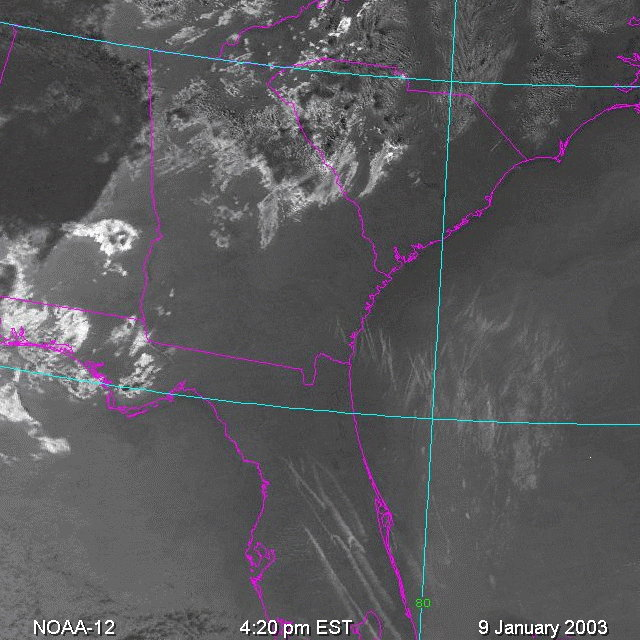
\includegraphics[scale=0.5]{pic/figure1.jpg}
\caption[Short form for the mapping directory]{"figure1.jpg"}
\label{figure1}
\end{figure}
Our program is inefficient for processing large images. The 
strategical removal of non-line edgels is computationally expensive.

  \chapter{Approach}

\section{Solution Strategy} 

This project’s goal is to distinguish contrails from the clouds, so we started by thinking about the main difference between the graphs of contrails and clouds. \\
Contrails usually show as a line on the image. Meanwhile, the clouds layout in a random discrete distribution. In this way, we can write a program to detect the straight lines in images to recognize the contrails. \\
However, it should be realized that even when the contrails look like pencil lines on the image, there doesn’t exist an actual straight line when scanning through the image data. Contrails also have some width in the image (in the real world, contrails could be several kilometers in width (CONTRAILS FACTS, page 3)). The real shape of contrails seems more like some long and thin rectangles with two fading sides. In this case, the detection problem became much harder. \\
Since this solution is hard to compute, instead of detecting the contrails’ width, it is much easier to just detect the two clear sides of contrails. In this case, we can ignore the image inside the contrails, as well as other pixels inside the cloud by doing the edge detection.\\
After performing the edge detection, we can detect lines by Hough Transform on the edgel map. Another problem was that there were too many edge pixels in the image (see the result by … below). Those bad edgels came to the Hough Transform to give incorrect lines, which do not come from contrails.\\
To solve this problem, some processing on the edge image to get rid of bad edge pixels is necessary. In order to delete those bad edge pixels from clouds or other graphics, each pixel with a certain size of pixels around is checked as a small block. As lines can be divided into infinity small lines, if a line goes through a small block, there must exist a small line inside the small block. We can use polynomial curve fitting to get the slope of the best small line in each block. Then we check how well the block edgels fit the computed line. Poor fits not as determined by a line residue causes the create edgel on the block to be rejected from the further Hough Transform.\\
After this processing, use the Hough Transform, a much better result will be got.\\

Here is the whole solution:

\begin{enumerate}
    \item Convert the color image to gray-scale;
    \item Use the Canny edge detection to get the edge;
    \item Get the small blocks pixel by pixel, and do the polynomial curve fitting to get the small line information;
    \item Put all the edgels surviving the polynomial curve fitting procedure into a new image;
    \item Do the Hough Transform on new image;
    \item Median filter the new image;
    \item Plot the results.
\end{enumerate}

\section{MatLab Methods}


\subsection{Canny Edge Detection}
\vspace{3mm}
\textit{Edge\_image = edge (I, \lq{canny}\rq);}\\
\newline
\textbf{Input: I, grayscale Image}\\
\textbf{Output: Edge\_image, the black and white edge image}\\
\newline
Canny edge detection is a technique to extract useful structural information from different vision objects and dramatically reduce the amount of data to be processed. There are following steps:
\begin{enumerate}
\item Apply the Gaussian filter to remove the noise;
\item Find the intensity gradient of the image;
\item Apply non-maximum suppression to get rid of spurious response to edge detection;
\item Apply double threshold to determine potential edges to filter out the edge pixel with the weak gradient value and preserve the edge with the high gradient value;
\item Track edge by hysteresis: Finalize the detection of edges by suppressing all the other edges that are weak and not connected to strong edges.
\end{enumerate}


\subsection{Polynomial curve fitting}
\vspace{3mm}
\textit{p = polyfit(x,y,n);}\\
\newline
\textbf{Input: \\x and y, vectors containing the x and y data to be fitted;\\ n, the degree of the polynomial to return;}\\ 
\textbf{Output: p, the third-degree polynomial that approximately fits the data.}\\
\newline
This algorithm returns the coefficients for a polynomial p(x) of degree n that is the best fit (in a least-squares sense) for the data in y. The coefficients in p are in descending powers, and the length of p is n+1.


\subsection{Hough Transform and Hough Line Transform}
\begin{wrapfigure}{r}{5.5cm}
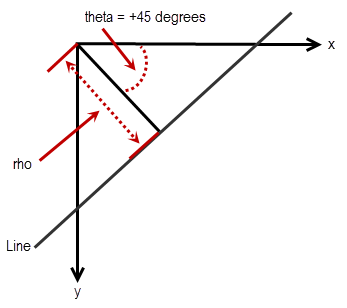
\includegraphics[width=5cm]{pic/SHT-example.png}\\
\caption{theta($\theta$) and rho($\rho$) of Hough Transform}
\end{wrapfigure}
\vspace{3mm}
\textit{[H,theta,rho] = hough(BW);}\\
\newline
\textbf{Input: BW, the black and white image;}\\
\textbf{Output:\\ H, the Hough Transform matrix be returned as a numeric array;}\\ 
\textbf{theta($\theta$), the angle in degree between the x-axis and rho vector;}\\
\textbf{rho($\rho$), the distance from origin to the line along a vector perpendicular to the line;}\\
\newline
The Standard Hough Transform (SHT) uses the parametric representation of a line: \begin{center} $\rho$ = xcos$\theta$ + ysin$\theta$.\end{center} 
For each pixel of the image, numbers of lines going through it with all different angles. If they are in the same line, they will have the same rho and theta number. During the graph or different angle and distance, we will get a cross point, which means the straight line’s rho and theta.\\ 
\begin{figure}[ht]
    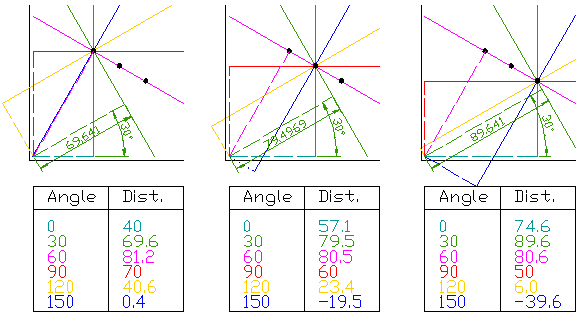
\includegraphics[scale=0.7]{pic/SHT-example2.png}
    \caption{$\theta$=60, $\rho$ are same for the 3 points}
\end{figure}
As we can see from above figure (Wikipedia.com), when the Hough Transform algorithm goes through all different angles ($\theta$) in every pixels, there is a certain angle ($\theta$ = 60 in above figure), it makes the perpendicular distance from the line to origin keeps the same ($\rho$ = 81.2 ~= 80.5 ~= 80.6). When we draw all the information below, we can have a much clear view for how the Hough Transform works.\\

\subsection{Median Filter}
\vspace{3mm}
\textit{B = medfilt2(A, [m n]);}\\
\newline
\textbf{Input:\\ A, the original image;}\\
\textbf{[m n], the isolate pixels’ size to be deleted;}\\ 
\textbf{Output: B, the image after deleted the isolated pixels.}\\
\newline
Put m x n pixel values around each target pixel into an array, then order all the values in the array, after this, we find the median value of the array and put it into the target pixels.

\section{Algorithm to reduce the bad edgels}

\subsection{Describe}
\textbf{This is a script, the input will be the edge image, and the output will delete the little block contains the small enough residual values.}\\
Since the Canny edge detection gives many edgels we need to further process these edge maps to eliminate edgels (edge pixels) that are not parts of straight lines. For each $2\times s$+1 by $2\times s$+1 square neighborhood about a pixel, we fit all the neighborhood edgels to a straight line using polyfit. We fit either y=mx+b for lines where $\left|m\right|$ $\leq$ 45 degrees and x=$\frac{y-b}{m}$ if $\left|m\right|$ $\geq$ 45 degrees. This takes care of horizontal and vertical lines. Now we have the equation of the best line fit for all the edgels in a neighborhood. But how good is this line fit? For each neighborhood edgel we compute the residual of that edgel’s neighborhood fit to the line. We compute the overall residual as the square root of the sum of these squared residual values.\\
Since neighborhoods with poor line fits will have large overall residual values, we remove bad edgels using a threshold of 15 determined by trial and error.

\subsection{Pseudo code}
\begin{lstlisting}[language=Java]
I = Read image;
grayscale (I);
image = Canny edge detect(I);
set the block size, height and width (s, height, width)
	
initial number no lines = 0;

for x = (1+s) to (height-s):
    for y = (1+s) to (width-s):
    initial points number = 0:
        if pixel is on an edge:
            for i = (x-s) to (x+s):
                for j = (y-s) to (y+s):
        	        if block pixel is edge:
                        record them;
                        points number ++;
        	if at least one line in a block:
        	    m = polyfit (x and y data recoded);
        	    if (line’s slope >1 or <-1):
        	        compute the residual r;
        	    else:
        	        modify the m;
        	        compute the residual r;
        	    save r values
        	else:
                number no lines ++;
                
get non_zero_r;
sort non_zero_r;	
set the precentage p;
threshold = cast(p% * non_zero_r);


for x = (1+s) to (height-s):
    for y = (1+s) to (width-s):
        if the r value is in the shreshold and non zero:
	        write it on new_image;
	        
new_image = medfilter (new_image);
get Hough Transform matrix(H), theta(T) and rho(R) by hough(new_image);
get peaks(P) = houghpeaks (new_image);
lines = houghlines(new_image, T, R, P);

for k = 1 to number of lines:
    plot lines on origin image(I);

\end{lstlisting}
  \chapter{Result}

\section{Best Result and Parameters}
\subsection{figure1}


\section{Discussion}


\section{Effect of Parameters}



\section{Problems}
This project solution still has some problems:
\begin{enumerate}
\item Some parameters need to be manually set if the best result is to be obtained, such as the canny edge threshold; the block size; the r value threshold; and Hough Transform minimum length, minimum gap, line numbers. Otherwise, the results would surprise some details when processing the multiple contrails images.
\item The images with multiple contrails that cross each other will be not be processed well because some blocks which have multiple contrails image cross each other might be deleted because of too large r value.
\item Super large image will be processed very slow because of the pixel by pixel processing algorithm. For example, figure4’s size is 2768 x 1845, and it took 1902 seconds (31.7 minutes) to process it (details see this project package /rst/figure4.txt). 
\end{enumerate}
  \chapter{Future Work}

Further work is needed to solve the problems that exist in current solution. Here are two directions to improve the program to make it more efficient: easier to use and faster to process the image.:
\begin{enumerate}
\item Automatically set some parameters, such as the parameters for Canny edge detection, block size, or r value threshold, etc. 
\item Use the MatLab’s parallel processes computing to reduce the loop processing time.
\end{enumerate}
  \chapter{Conclusion}

This project is designed to recognize the contrails from clouds image. Using 
Canny edge detection, polynomial curve fitting, and the Hough Transform (all
via MatLab) we have proposed a solution to problem. The algorithms we developed are:
\begin{enumerate}
\item Convert the original image to grayscale,
\item Use the Canny edge detector to compute edge maps,
\item Processing small blocks edgel by edgel and performing polynomial curve fitting 
to obtain the best small line fit in each block and then thresholding edgels 
based on the residual of the line fit,
\item Placing edgels that survive this residual thresholding into into a new image,
\item Performing a Hough Transform on new edgel image to extract significant lines and
\item Plotting the results.
\end{enumerate}
From the results, it can be seen that the problem has been fairly well solved. 
However, some problems still exist, such as parameters setting, good data that 
was missed or deleted, and computational time issues.

We can still do some further research on solving this problem, for example, 
making the program more efficient or easier to use.

  





	\begin{figure}[hbtp]
		\centering
		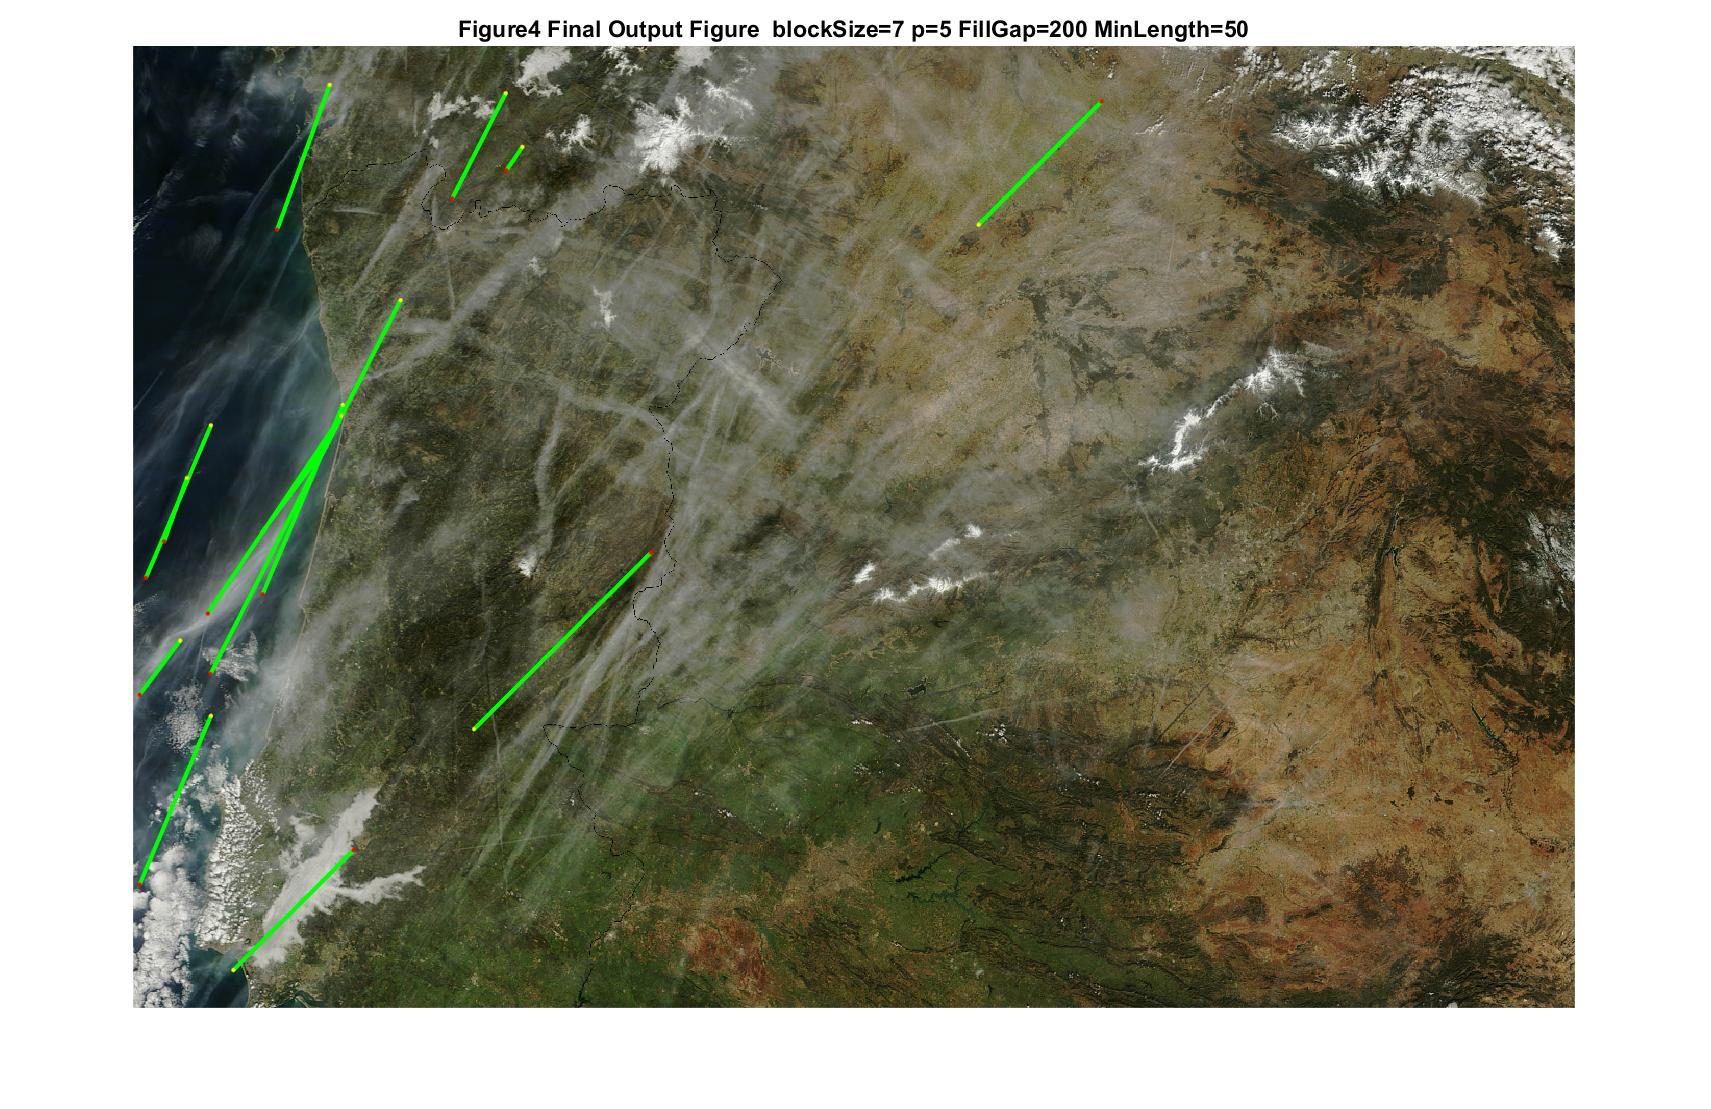
\includegraphics[width=6in]{pic/Figure4_best.jpg}
		\caption{Best Result for Figure \ref{figure4}}
		\label{Figure4_best}
	\end{figure}


	\begin{figure}[hbtp]
		\centering
		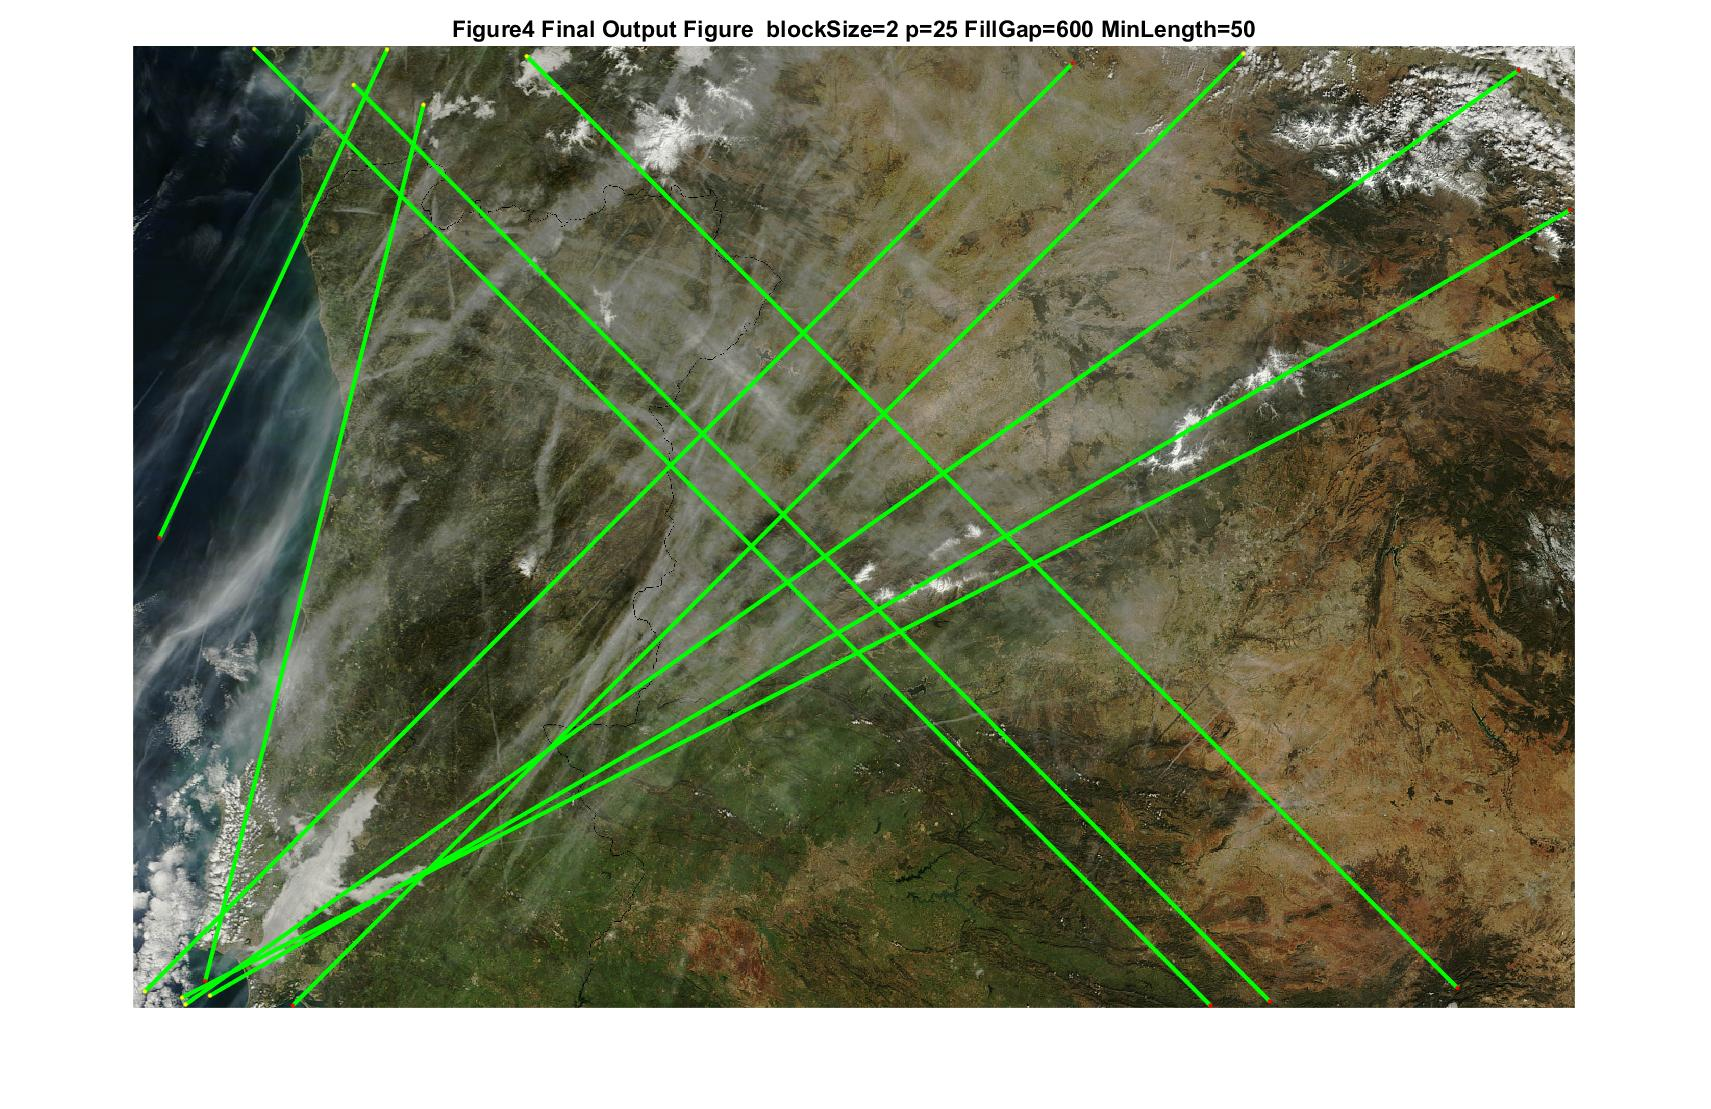
\includegraphics[width=6in]{pic/Figure4_worst.jpg}
		\caption{Best Result for Figure \ref{figure4}}
		\label{Figure4_worst}
	\end{figure}


	\begin{figure}[hbtp]
		\centering
		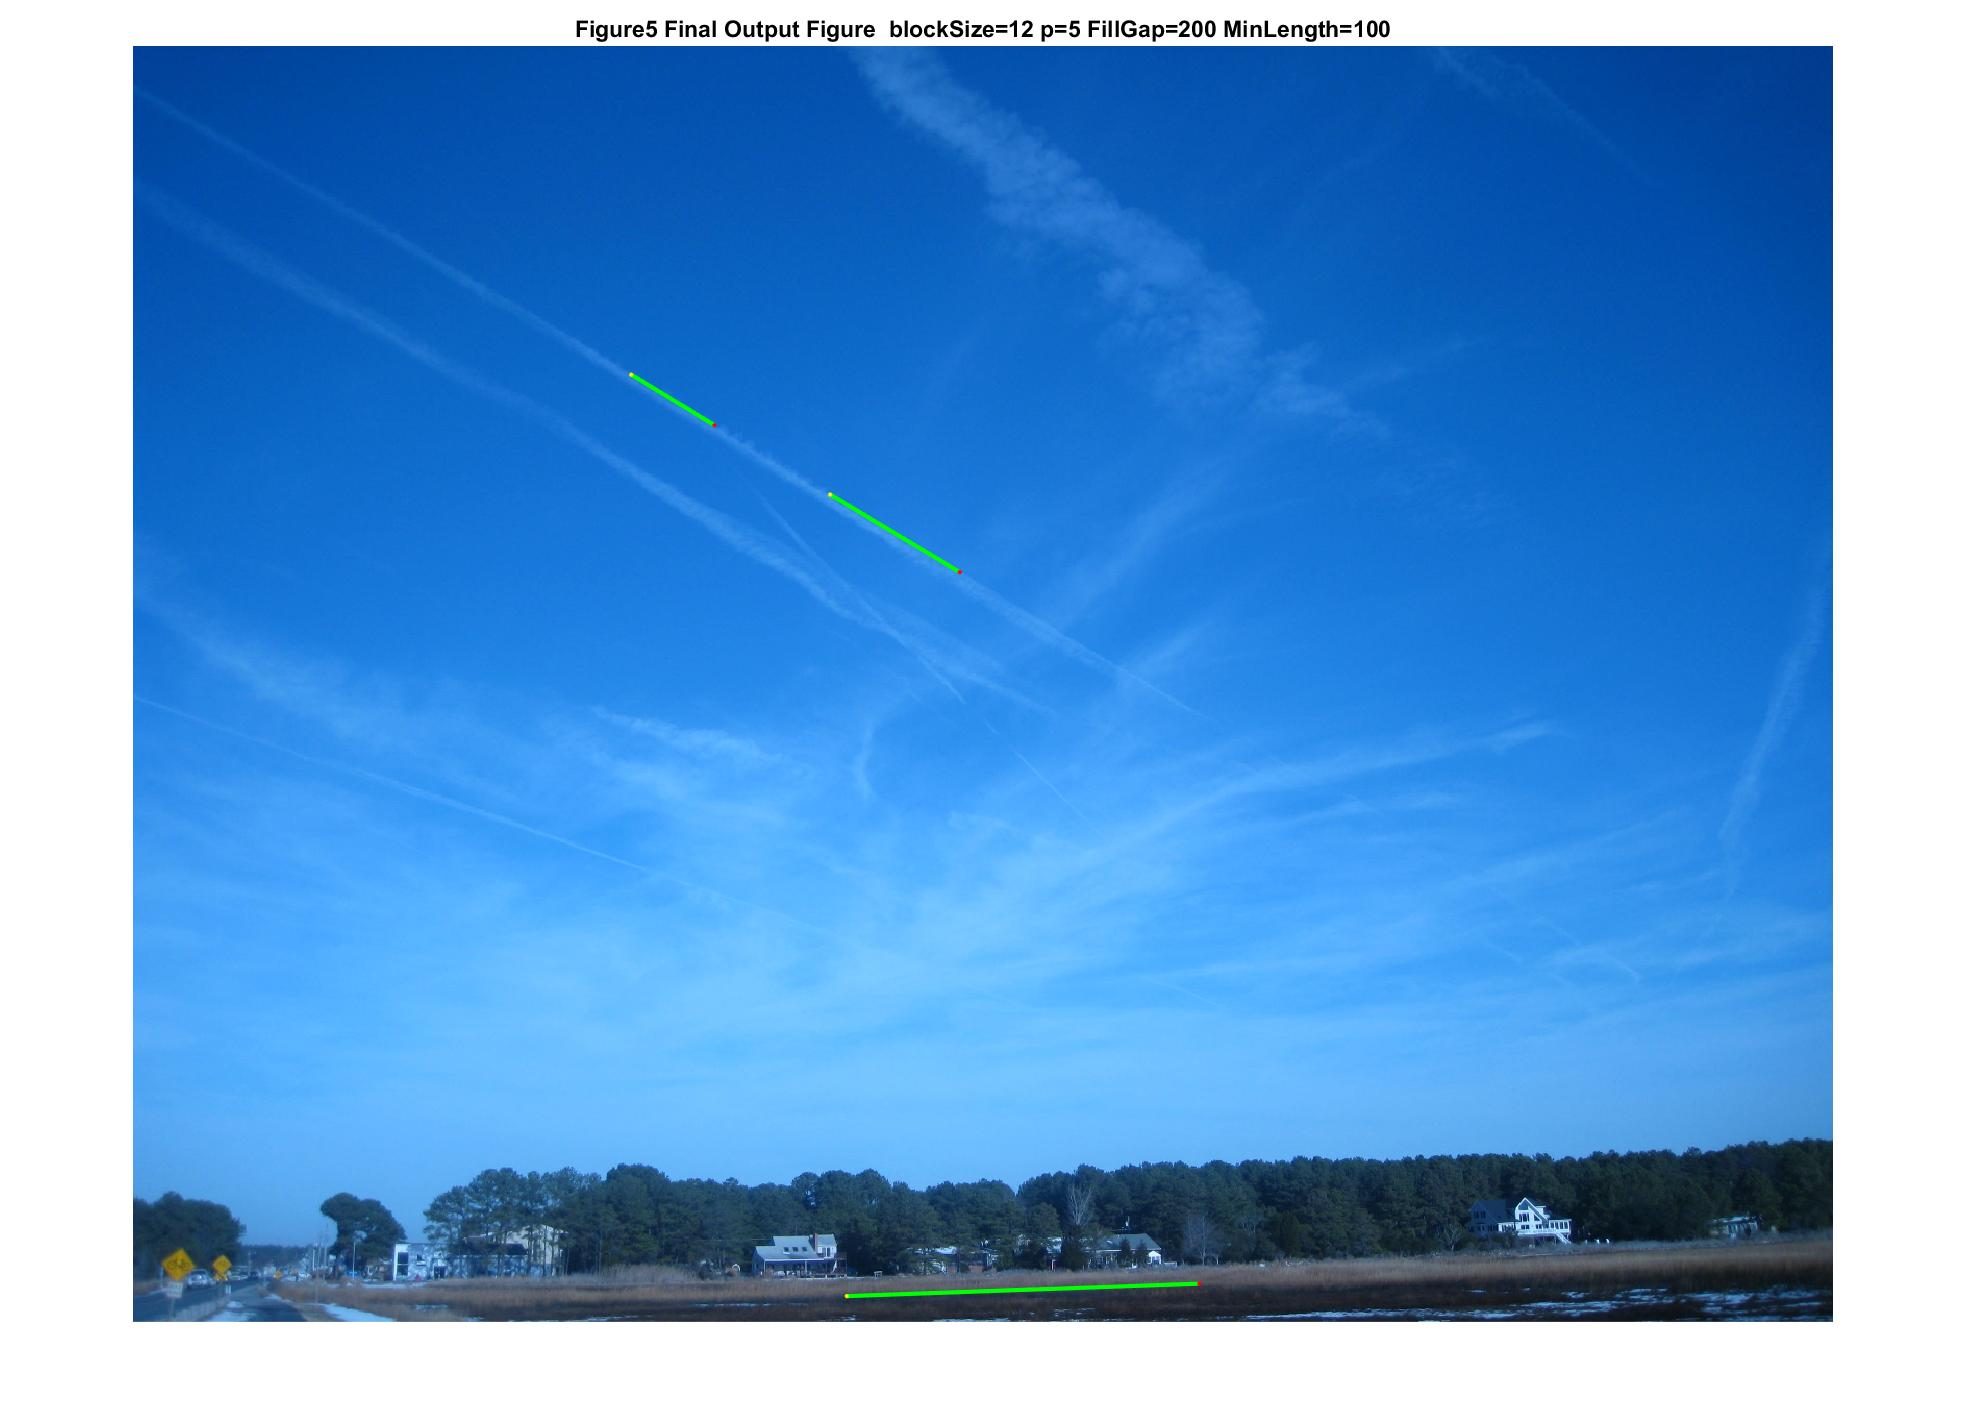
\includegraphics[width=6in]{pic/Figure5_best.jpg}
		\caption{Best Result for Figure \ref{figure5}}
		\label{Figure5_best}
	\end{figure}


	\begin{figure}[hbtp]
		\centering
		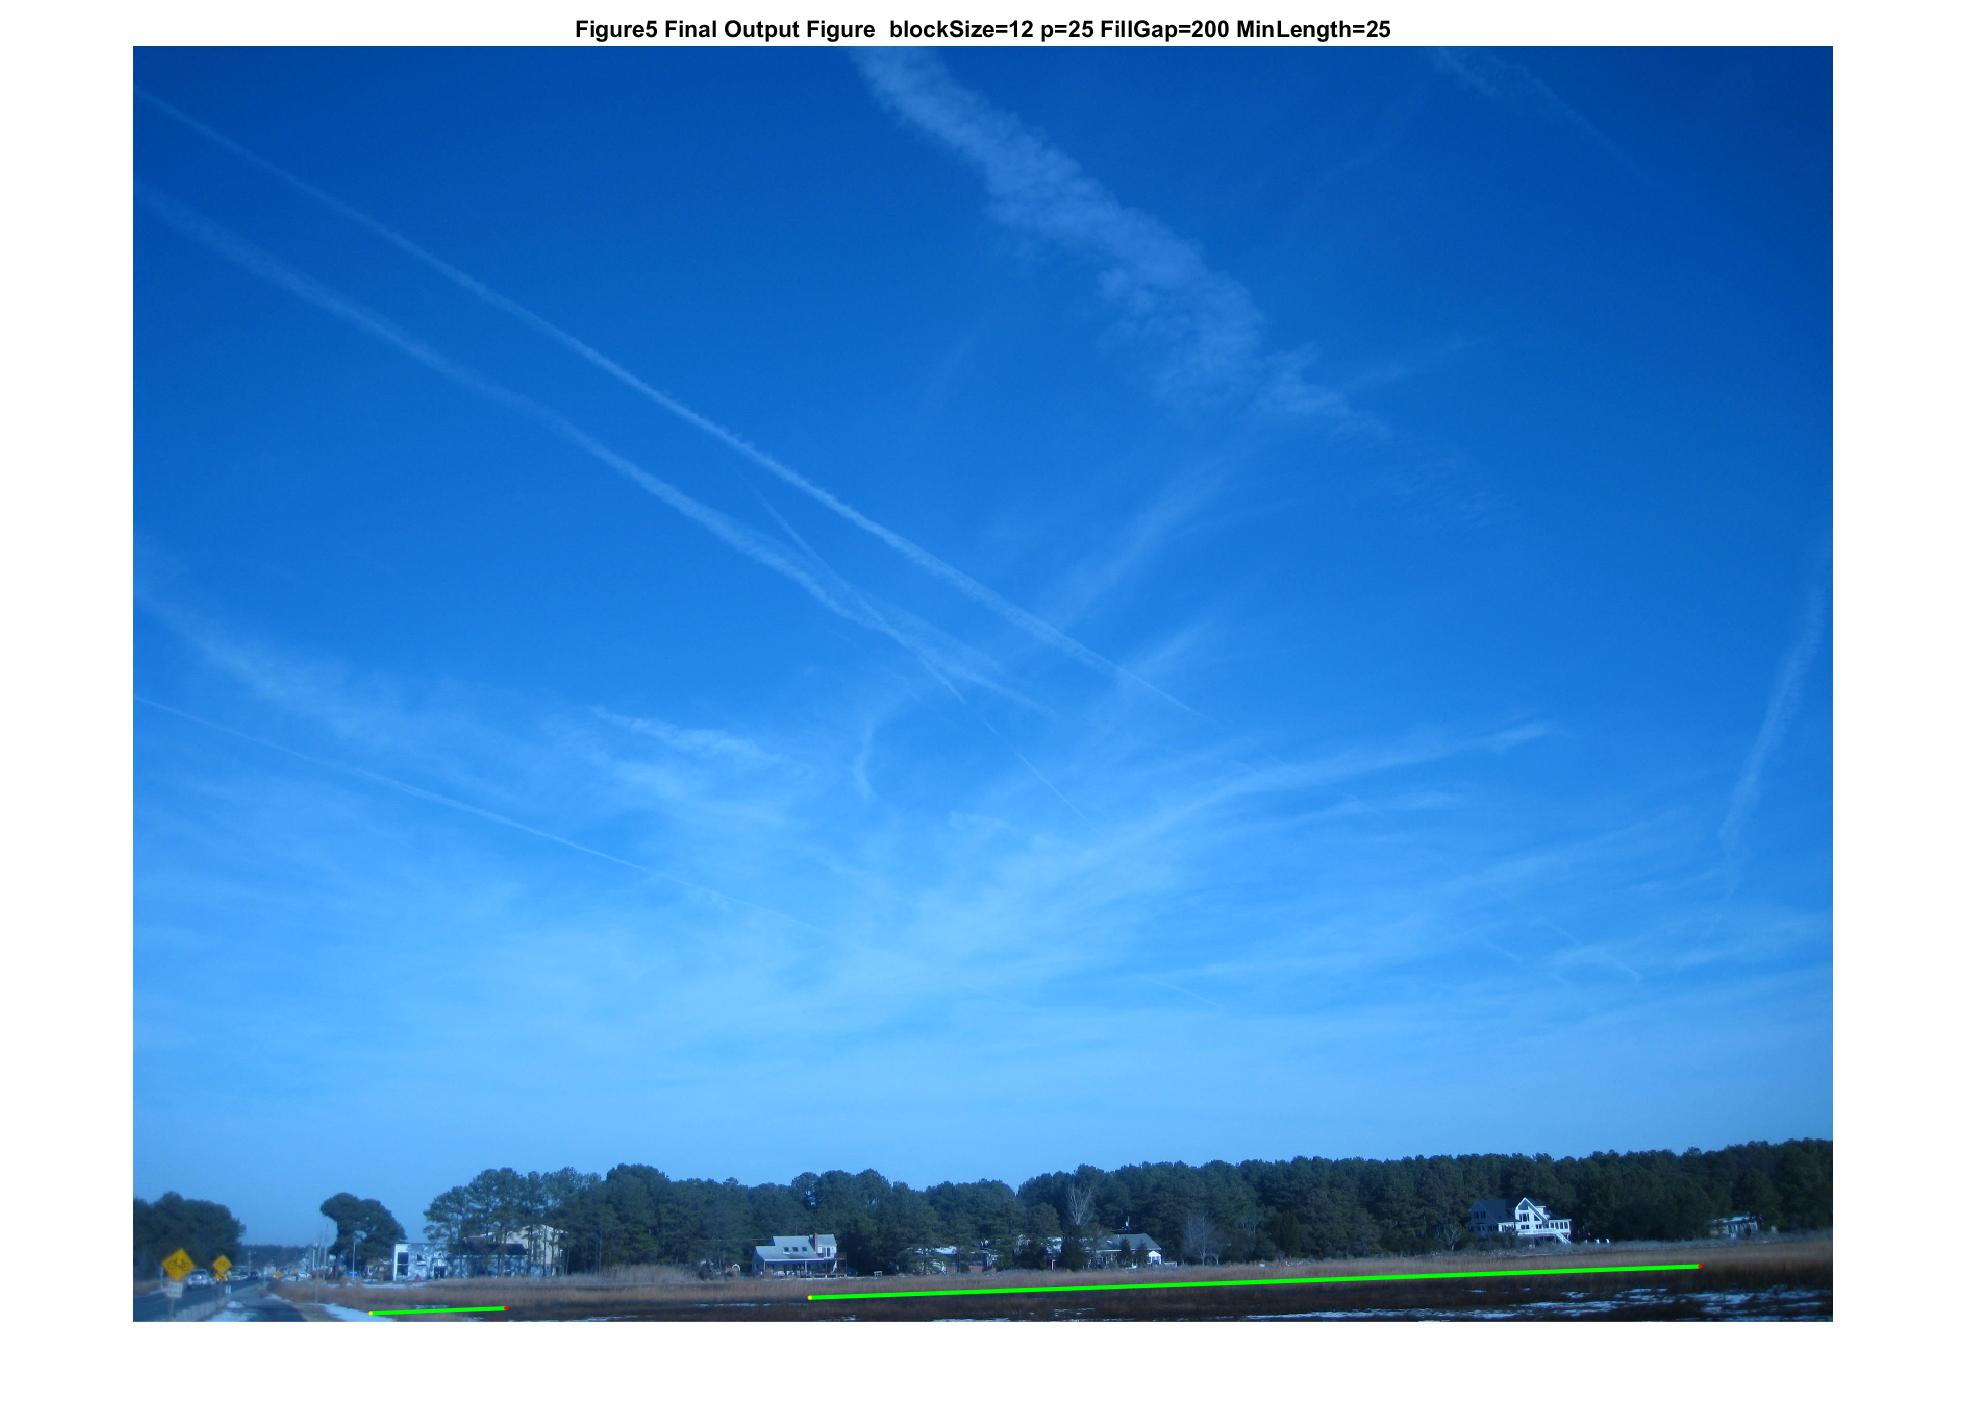
\includegraphics[width=6in]{pic/Figure5_worst.jpg}
		\caption{Best Result for Figure \ref{figure5}}
		\label{Figure5_worst}
	\end{figure}



  \backmatter
  \include{bibliography}
  \markboth{}{}


  \addcontentsline{toc}{chapter}{\protect thanks}


\chapter*{thanks}

Danke.



  \chapter*{curriculum vitae}

Sigmund Stintzing

\vspace*{2.0cm}

\begin{tabular}{ll}

Geburtsdatum & Geburt in Geburtsort \\[1.5ex]
Schulzeit & Besuch der Schule in Ort \\[1.5ex]
 ... & ...
\end{tabular}



\end{document}
